
Auf Basis der in der Balkenberechnung bestimmten Parameter Biegesteifigkeit, maximales Biegemoment und der maximalen Querkraft, sollen die Gurte und der Steg dimensioniert werden. Die Vorauslegung soll dabei anhand der VDI- Richtlinie 2013 erfolgen, diese enthält in einem Unterkapitel Informationen speziell zur Auslegung eines I-Trägers. Dabei ist zu beachten, dass bei einigen Berechnungen Vereinfachungen angenommen werden, die an den betreffenden Stellen spezifiziert werden. Zusätzlich sei angemerkt, dass die erste Auslegung nur an an ausgewählten Stellen Sicherheitsfaktoren ungleich eins berücksichtigt. Grund dafür ist die Annahme, dass in den bereitgestellten Materialkennwerten ausreichende Sicherheiten verrechnet worden sind.

\subsection{Dimensionierung der Gurte}
\begin{figure}
	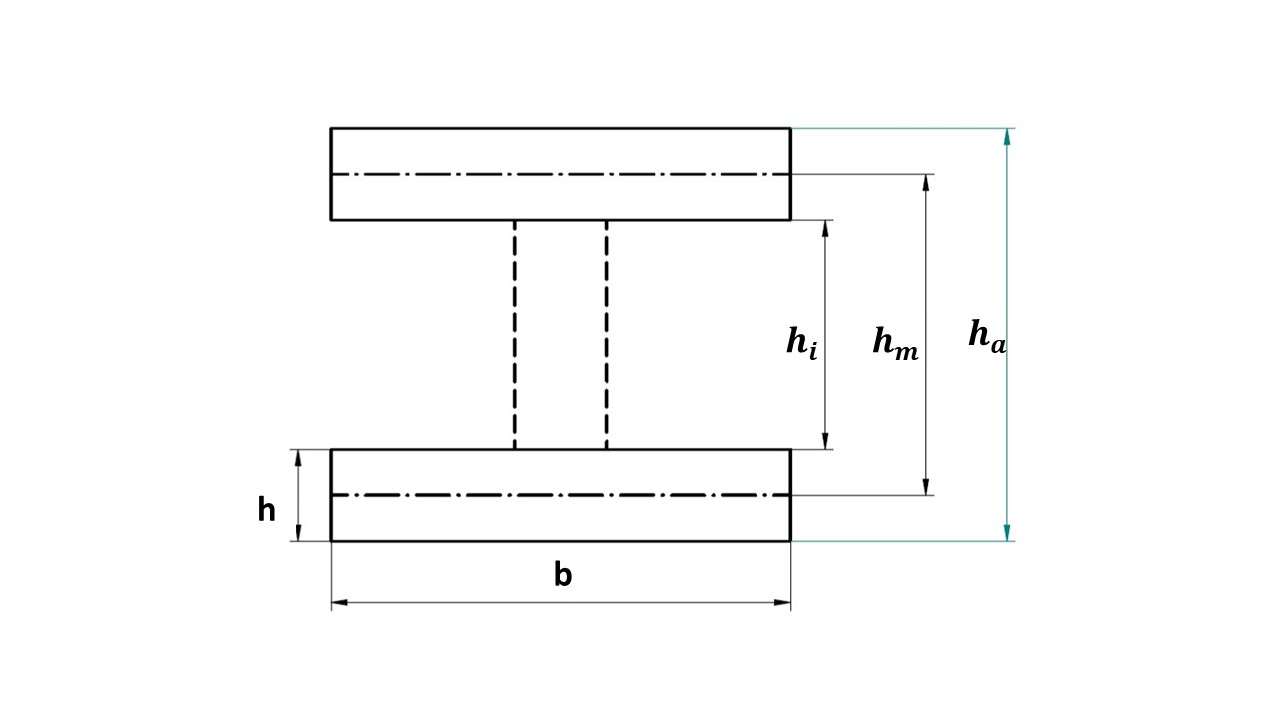
\includegraphics[width=1.0\textwidth]{Bilder/RechteckHolm.jpg}
	\caption{Maße des rechteckigen I-Holms}
	\label{fig: Rechteckholm}
\end{figure}

Bei der Auslegung der Gurte auf Steifigkeit wird angenommen, dass der Steg des I-Trägers keine Längskräfte aufnimmt und der Biegung nicht entgegenwirken kann. Die in der Balkenberechnung ermittelte Biegesteifigkeit $ EI_{x} = 952,55 Nm^{2} $, die erforderlich ist, damit bei einer Kraft $ F_{pruef}=100N $ die Flügelspitze eine Absenkung von $ w_{j=1,1}=20mm $ erfährt, muss allein durch die Gurte aufgebracht werden. Im Sinne der kraftflussgerechten Gestaltung sollen die Glasfasern unidirektional in Längsrichtung des Gurtes angeordnet werden. Die Bezeichnungen der Längenangaben des Holmes orientieren sich an Abb.~\ref{fig: Rechteckholm}~.\\



\noindent Die Gurte werden zur Bestimmung der notwendigen Lagenanzahl als rechteckig angenommen, erst in einem späteren Schritt soll die Form der Kontur der vorgegebenen Haut angepasst werden. Die Maße sind über die gesamte Länge des Holms als konstant anzusehen.\\
Zur Bestimmung des Flächenträgheitsmomentes $ I_{x} $ wird der E-Modul in Längsrichtung der Fasern nach der Mischungsregel nach [3] berechnet.\\
\begin{equation}
 E_{11}=  \phi*E_{f,11}+\left( 1-\phi \right) * E_{M}
\end{equation}
Mit den gegebenen Materialkennwerten bestimmt sich $ E_{11} = 31580 MPa $. Damit ergibt sich ein benötigtes Flächenträgheitsmoment von $ I_{x} = 3,01631 * 10^{-8} m^{4} $.\\

\noindent Das Flächenträgheitsmoment der Gurte bestimmt sich aus den Flächenträg-heitsmomenten der beiden Rechteckquerschnitte und ihren zugehörigen Steiner-Anteilen.
\begin{equation}
	\label{Ix}
	I_{x}=2*\left(\frac{b*h^{3}}{12}+b*h*\left(\frac{h_{m}}{2}\right)^{2}\right)
\end{equation}

\noindent Es wird nach einer Kombination aus Gurtbreite $ b $ und Gurthöhe $ h $ gesucht, die die Anforderungen an das Flächenträgheitsmoment erfüllt, aber dennoch zu einer möglichst geringen Gurtquerschnittsfläche und damit zu einer möglichst geringen Masse der Gurte führt. Um die Steiner-Anteile der Gurte zu maximieren, sollen die Gurte in einem möglichst großen Abstand zur neutralen Faser angeordnet werden. Vorgegeben ist eine Profildicke von $ 37,5mm $, allerdings muss berücksichtigt werden, dass die nach innen gelegte Haut, die Wölbungsrücklage und die Dickenrücklage die maximale Höhe des Holmes einschränken. Deshalb wird die gesamte Gurthöhe auf $ h_{a}=36mm $ abgeschätzt.\\ 

\noindent Die nachstehende Tabelle ~\ref{bh} enthält Werte der Gurtquerschnittsfläche bei verschiedenen Kombinationen von $ b $ und $ h $, die zu einem gesamten Flächenträg-heitsmoment von $ I_{x} = 3,01631 * 10^{-8} m^{4} $ führen.\\
\begin{table}
	\caption{Verschiedene Kombinationsmöglichkeiten von $ b $ und $ h $}
	\label{bh}
	\begin{center}
		\begin{tabular}{l|c|r}
			$h$&$b$&$2*b*h$\\
			\hline
			$1mm$&$38,3mm$&$76,6mm^{2}$\\
			$1,25mm$&$31,1mm$&$77,7mm^{2}$\\
			$1,5mm$&$26,3mm$&$78,8mm^{2}$\\
			$2,25mm$&$18,3mm$&$82,3mm^{2}$\\
		\end{tabular}
	\end{center}
\end{table}

\begin{figure}
	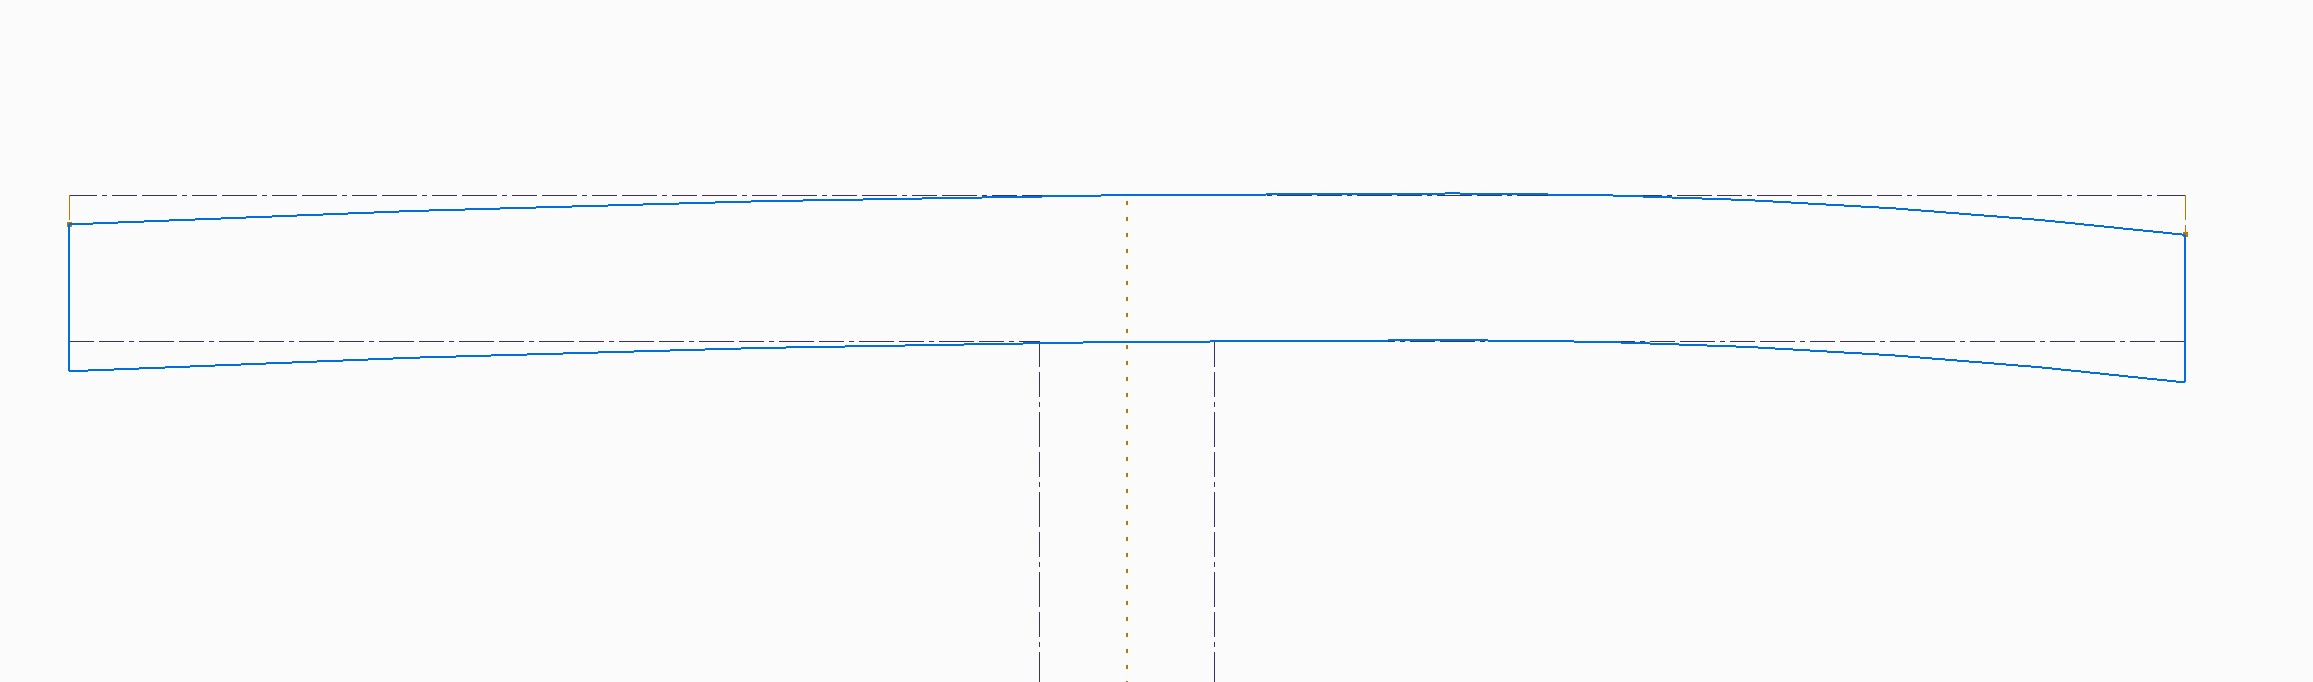
\includegraphics[width=1.0\textwidth]{Bilder/KrummerGurt.jpg}
	\caption{Der rechteckige Gurt ist gestrichelt dargestellt, der angepasste gekrümmte Gurt mit einer durchgezogenen Linie.}
	\label{fig: KrummerGurt}
\end{figure}


\noindent Den Daten ist zu entnehmen, dass breite Gurte geringer Dicke bei gleichem Flächenträgheitsmoment geringere Querschnittsflächen aufweisen. Aus diesem Grund sollen die Gurte möglichst breit gewählt werden. Die Breite der Gurte ist durch die vorgegebene Konstruktion der Platte zur Aufnahme der Tragfläche am Teststand begrenzt. Die vorgesehene Aussparung weist eine Breite von $ 30mm $ auf. Für die weitere Berechnung soll $ b=28mm $ gelten. Diese Annahme wird dadurch begründet, dass die Fertigung des Holms im Bereich des Modellbaus von Hand erfolgen würde, womit nur grobe Toleranzen einhaltbar sind.\\

\noindent Mithilfe eines Solvers bestimmt sich aus dem Flächenträgheitsmoment und der Gurtbreite die Gurthöhe $ h=1,845mm $.\\
\noindent Im nächsten Schritt wird die zu stapelnde Lagenanzahl ermittelt. Als unidirektionales Material steht das Glasgewebe Interglas 92145 mit einem Flächengewicht von $ 220\frac{g}{m^{2}} $zur Verfügung. Nach [3] berechnet sich die Lagenanzahl $ n $ für eine Dicke des Verbundes $ t_{soll} $ zu:\\

\begin{equation}
	\label{gurtlagen}
	n=t_{soll}*\frac{\phi*\rho_{f}}{\left(\frac{m_{f}}{L*b}\right)}
\end{equation}

\noindent Mit $ \left(\frac{m_{f}}{L*b}\right) = 220\frac{g}{m^{2}} $ und $ t_{soll}=h $ ergibt sich $ n=8,55 $. Es sind also 9 Lagen des Gewebes 92145 für jeden Gurt vorzusehen.Die sich aus 9 Lagen ergebende Gurthöhe kann durch Umstellen von Gleichung ~\ref{gurtlagen} zu $ \tilde{h}=1,941mm $ bestimmt werden. Für den zunächst angenommenen Fall von Gurten mit rechteckigen Querschnitten ist die Auslegung zur Einhaltung der Anforderungen an die Steifigkeit damit abgeschlossen.\\


\subsection{Nachrechnung der angepassten Gurte}
 Die Modellierung der Haut und der Holmgurte in einem CAD-Programm zeigt, dass die Gurte mit den berechneten Bemaßungen nicht innerhalb des Profils mit der als $ 0,75mm $ dick angenommenen Haut liegen. Die Anpassung der Konstruktion der Gurte erfolgt so, dass sich die Gurtoberseite der Innenseite der Haut anschmiegt.Die Gesamtbreite von $ 28mm $, sowie die Gurtdicke bleiben dabei gleich. Da die Wölbungsrücklage ungleich der Dickenrücklage ist, muss die Gesamthöhe $ h_{a} $ auf $ \tilde{h_{a}}=35,8mm $ leicht verringert werden. Abbildung ~\ref{KrummerGurt} veranschaulicht die gekrümmte Form des oberen Holmgurtes.\\
 
\noindent Die angepasste Krümmung der Gurte führt zu einem veränderten Flächenträg-heitsmoment $ \tilde{I_{x}} $ des Balkens, dass mithilfe des CAD-Programms exakt zu $ \tilde{I_{x}}=3,075406*10^{-8}m^{4} $ bestimmt werden kann. Da $ 3,075406*10^{-8}m^{4} > 3,01631*10^{-8}m^{4} $ ist, genügen auch die veränderten Gurte der Steifigkeitsanforderung. Abschließend wird gezeigt, dass die Festigkeit der Gurte einer Belastung der Flügelspitze durch $ F_{pruef}=500N $ standhält. Die aus der Biegung resultierenden und betragsmäßig gleichen Zug- und Druckspannungen werden dazu mit den vorhandenen UD-Festigkeitskennwerten des Handlaminats verglichen. Die Resultate der Balkenberechnungen zeigen, dass das maximale Biegemoment im Holm an Punkt C auftritt und $ M^{b}=500N*0,773m=386,5Nm $ beträgt.In den Randfasern der Gurte resultieren Spannungen, die sich nach\\
\begin{equation}
	\sigma_{b}=\frac{M_{b}*\tilde{h_{a}}}{\tilde{I_{x}}*2}
\end{equation} 
zu $ \sigma_{b}=224,96MPa $ berechnen. Da $ \sigma_{b}< R^{(+)}_{||}=597,9MPa < R^{(-)}_{||}=650,0MPa $, ist der Festigkeitsnachweis erbracht. Es kann davon ausgegangen werden, dass die Gurte bei einer Prüfkraft von $ F_{pruef}=500N $ nicht versagen. 
 

  
